
\subsubsection{Modell}
Die nummerische Analyse findet mit Hilfe des Programms ABAQUS des Anbieters Dassault Systemes statt. Das Programm ist für Studenten kostenlos erhältlich, jedoch ist diese Version auf eine Anzahl von 1000 Knoten beim Vernetzen des Bauteils beschränkt.\\
Das zuvor erstellte CAD-Modell wird zunächst in ABAQUS importiert. Da es sich nun zunächst noch um ein Vollmaterial handelt und für eine möglichst genaue Analyse ein Schalenmodell verwendet werden soll, muss das Modell zunächst umgewandelt werden.(siehe Abb. \ref{Schalenmodell})

\begin{figure}[h]
 \centering
 \includegraphics[scale=0.4]{Bilder/Flügel_ABAQUS}\\
 \label{Schalenmodell}
 \caption{Schalenmodell}
\end{figure}
\newpage

Daraufhin werden für die Materialien die Kennwerte in das Programm integriert. Hierbei werden die Werte für GFK, den Schaum und die Rippen eingetragen(siehe Abb.\ref{Material}).Diese wurden in Kapitel 4.3.1 mit Hilfe von elamX festgelegt.\\
\begin{figure}[h]
 \centering
 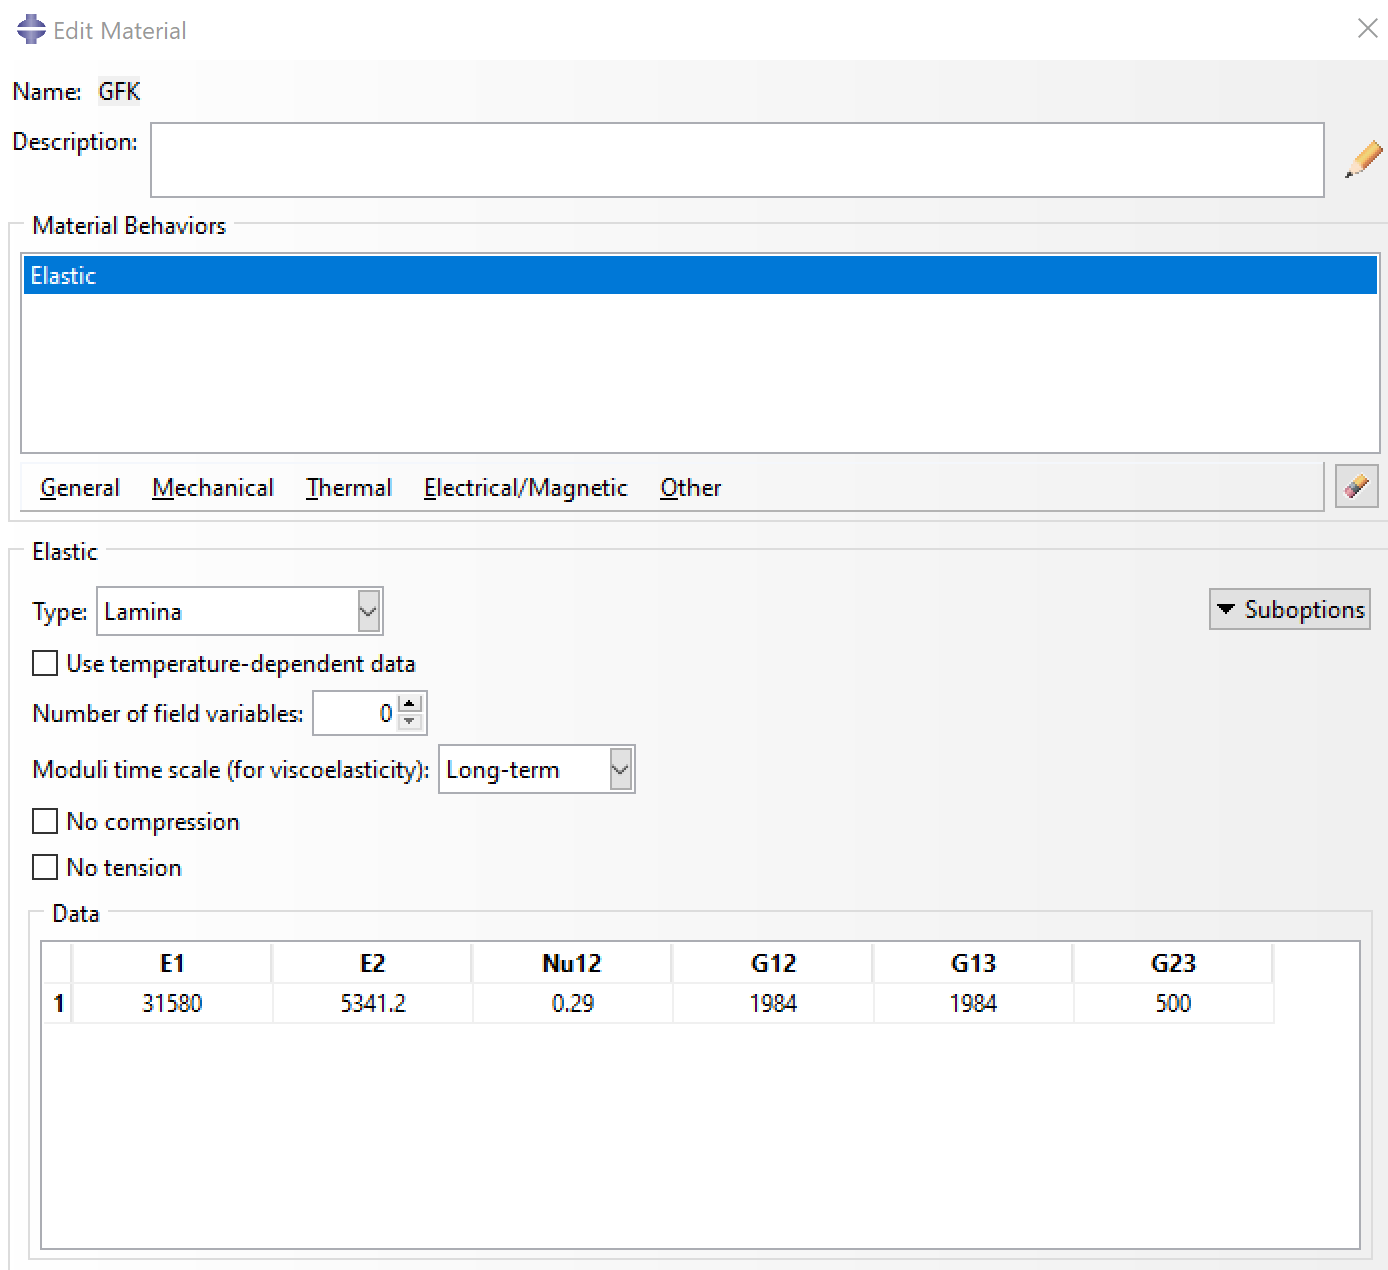
\includegraphics[scale=0.4]{Bilder/Material_GFK}\\
 \label{Material}
 \caption{Beispiel GFK}
\end{figure}
\newpage

Als nächstes wird das Schalenmodell in die Verschiedenen Segmente Unterteilt , denen dann Materialien und deren entsprechenden Dicken und Anzahl von Schichten zugeortnet. Hierbei wird das Bauteil in den Dicken und den dünnen Teil des Stegs,die Gurte,die Haut,sowie die Haut eingeteilt.(Materialdicken und Schichten nennen)
\begin{figure}[h]
 \centering
 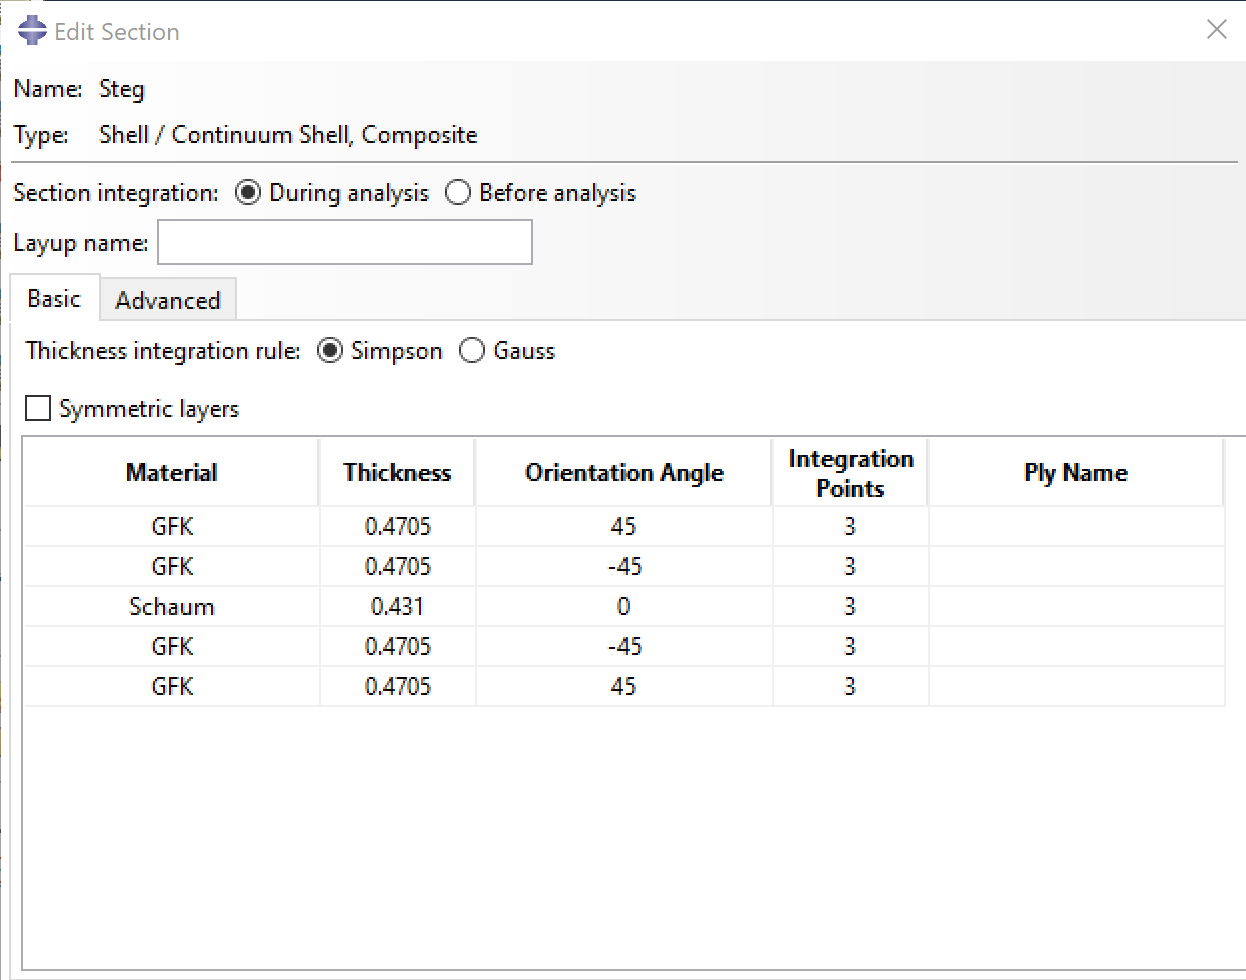
\includegraphics[scale=0.4]{Bilder/Steg_Material}\\
 \label{Steg_Material}
 \caption{Beispiel:Steg}
\end{figure}
Als nächstes werden die Randbedingungen und Angreifenden Kräfte festgelegt. Der Holm ist in der Einspannung fest gelagert. Daher wird an der Stelle der Lager A und B eine feste Einspannung angenommen. Die Aufgenommenen Kräfte durch die Querkraftbolzen werden als Kräfte angebracht.Die Prüfkraft wird am L/4-Punkt eingeleitet.

Daraufhin wird das Bauteil vernetzt. Hierbei wird eine Anzahl an Knoten pro Längeneinheit eingegeben und das Programm verbindet diese zu einem Netz aus Vierecken. Durch die Begrenzung auf 1000 Knoten ist das Netz jedoch recht grob. \\
\newpage
\subsubsection{Analyse}
Zunächst wird eine Prüfkraft von 100N angelegt, um die maximale Absenkung zu ermitteln. Hierbei ergibt sich für die Absenkung $z_{max}=17,34mm$. Dies ist weniger als die geforderte Absenkung von $z_{max}=22mm$ und somit kann dieses Aufgabenkriterium als erfüllt angesehen werden.
\begin{figure}[h]
 \centering
 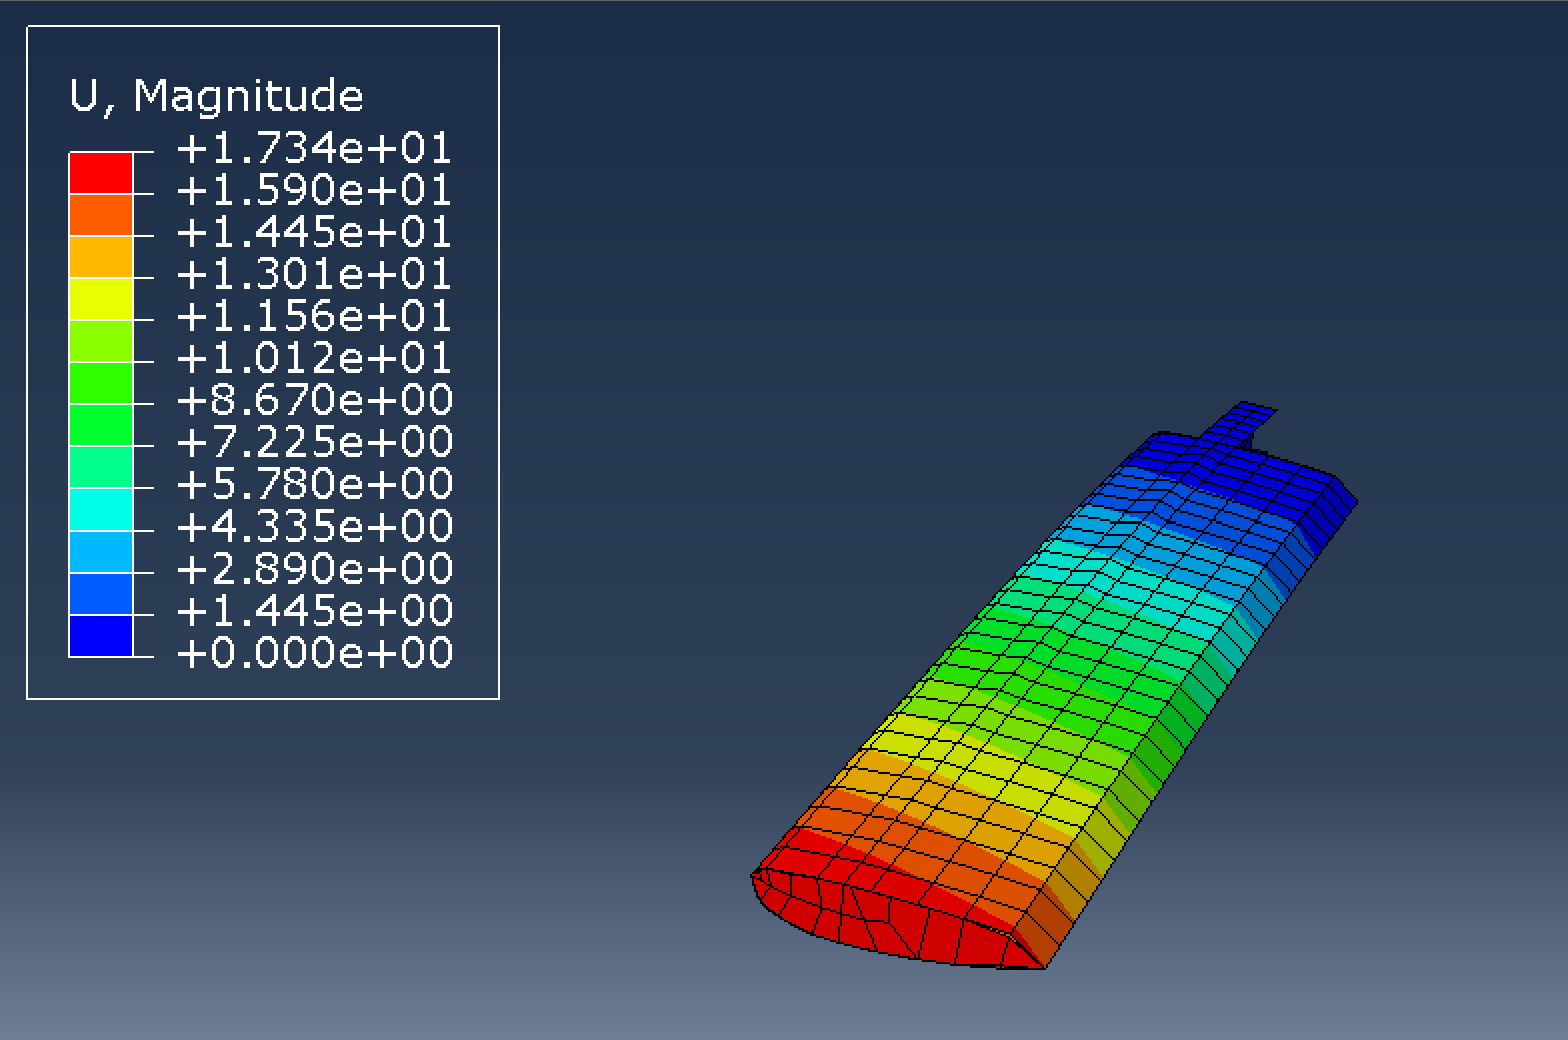
\includegraphics[scale=0.4]{Bilder/Absenkung_100N}\\
 \label{Absenkung}
 \caption{Absenkung bei einer Belastung von 100N}
\end{figure}
\newpage
Um herauszufinden, ob der Flügel einer Beanspruchung von 500N standhält wird die Prüfkraft auf 500N erhöht. Nun müssen die maximalen Spannungen im Bauteil mit den Kennwerten verglichen werden. Das Modell zeigt nun maximale Spannungen an der Stelle des Lagers B an. Da sich dort allerdings noch eine nicht mit modellierte Verstärkung durch Holzblöcke befindet sind diese Werte deutlich höher als in der Realität. Daher werden die Werte angenommen, die sich ab der Rippe ergeben.\\
 Die maximale Vergleichsspannung ergibt sich im Steg des Holms. Die Normalspannung in $x_{1}$-Richtung ist im vorderen Teil des Stegs am höchsten und beträgt beim Maximum $85,63\frac{N}{mm^2}$.\\
Die Normalspannung in $x_{2}$-Richtung ist im Gurt der Unterseite des Flügels (im Veruchsaufbau Oberseite) und beträgt maximal $14,25\frac{N}{mm^2}$.Die Spannung in $x_{3}$-Richtung ist überall 0.\\
Die Schubspannung ist in der Schale auf der Unterseite am höchsten. Hier ergibt sich ein Maximalwert von $16,72\frac{N}{mm^2}$.\\
Das Angenommene Koordinatensystem bezieht ich auf die oberste Schicht des Laminats. Daher sind $x_{1}$ und $x_{2}$ immer in Richtung der Faser oder orthogonal dazu.\\
Die Werte sind durch das Zusammenspiel aller Bauteile sehr viel kleiner als in den Vorherigen Berechnungen. Dadurch bestätigt das FEM- Modell die vorangegangenen Berechnungen.
\newpage
\subsubsection{Beulanalyse}
Da der Holmstummel bis zum Lager C nicht ausreichend modelliert werden konnte wird für die Beulauslegung eine feste Einspannung am Lager C angenommen.\\
\begin{figure}[h]
 \centering
 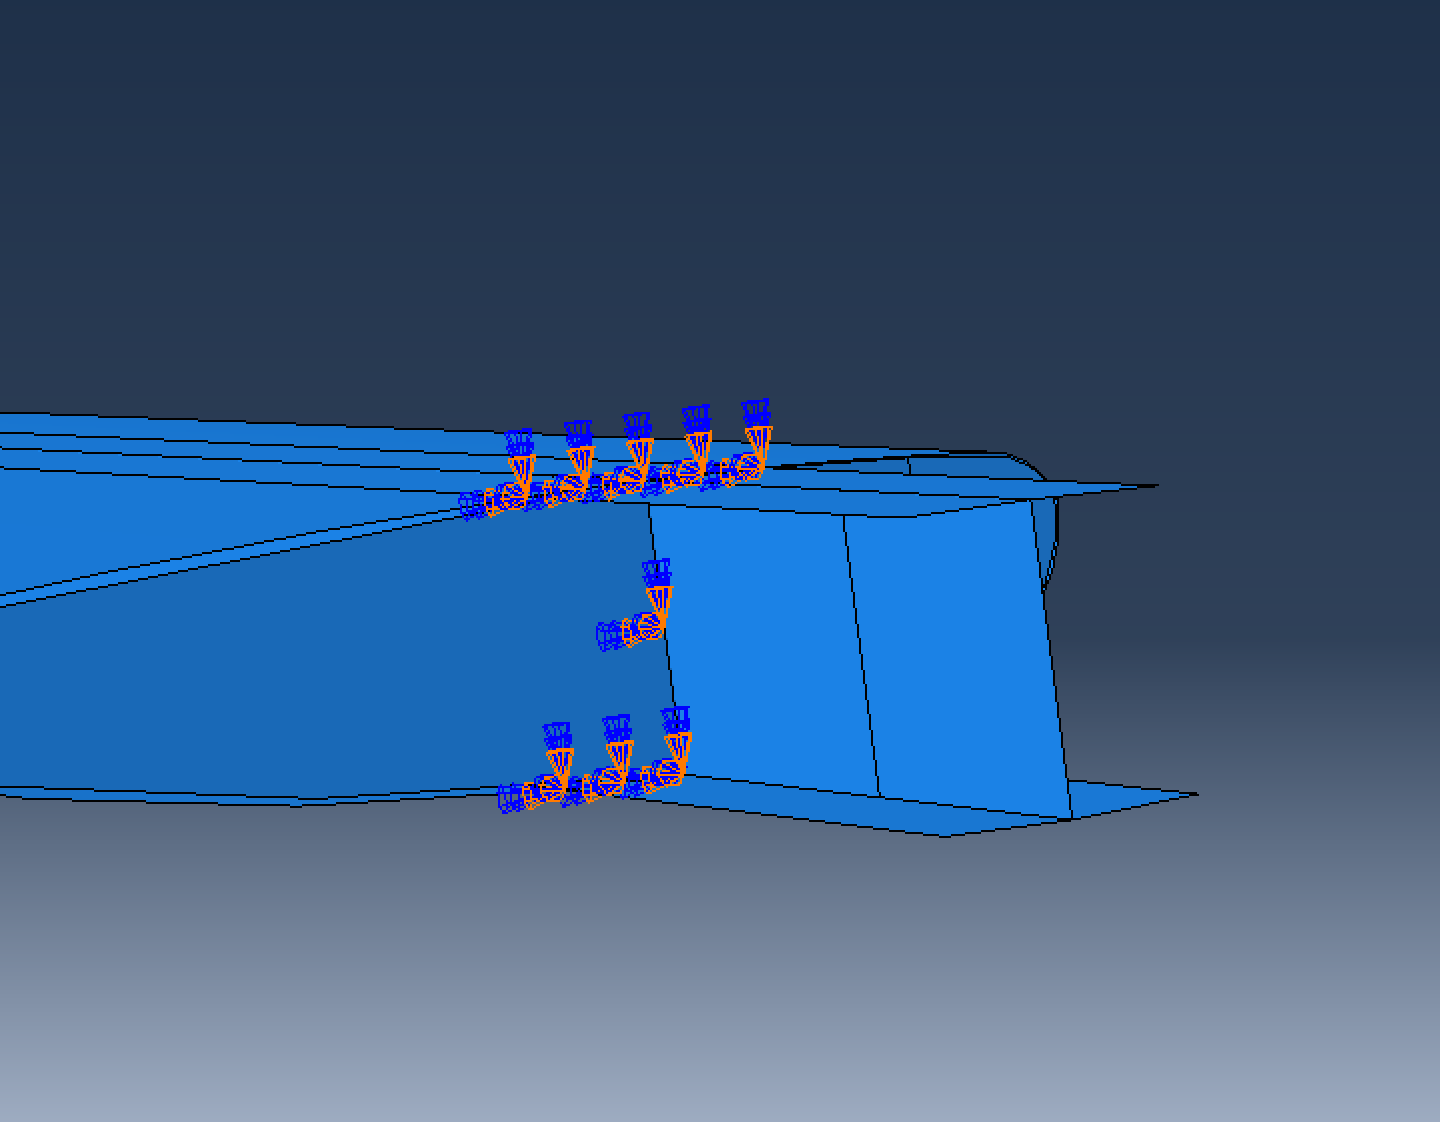
\includegraphics[scale=0.4]{Bilder/Beuleinspannung}\\
 \label{Absenkung}
 \caption{Einspannung am Lager C}
\end{figure}
Nun können die Eigenwerte für die Belastung von 100N, 500N und 1000N abgelesen werden.
\begin{center}
\begin{tabular}[h]{l|c}
Prüfkraft&Beulfaktor\\
\hline
100N&10,253\\
500N&2,0506\\
1000N&1,0253\\
\end{tabular}
\end{center}

Diese Werte sind alle größer als 1, damit ist der Flügel für alle drei Belastungsfällen ausreichend gegen das Beulen dimensioniert.\\
\begin{figure}[h]
 \centering
 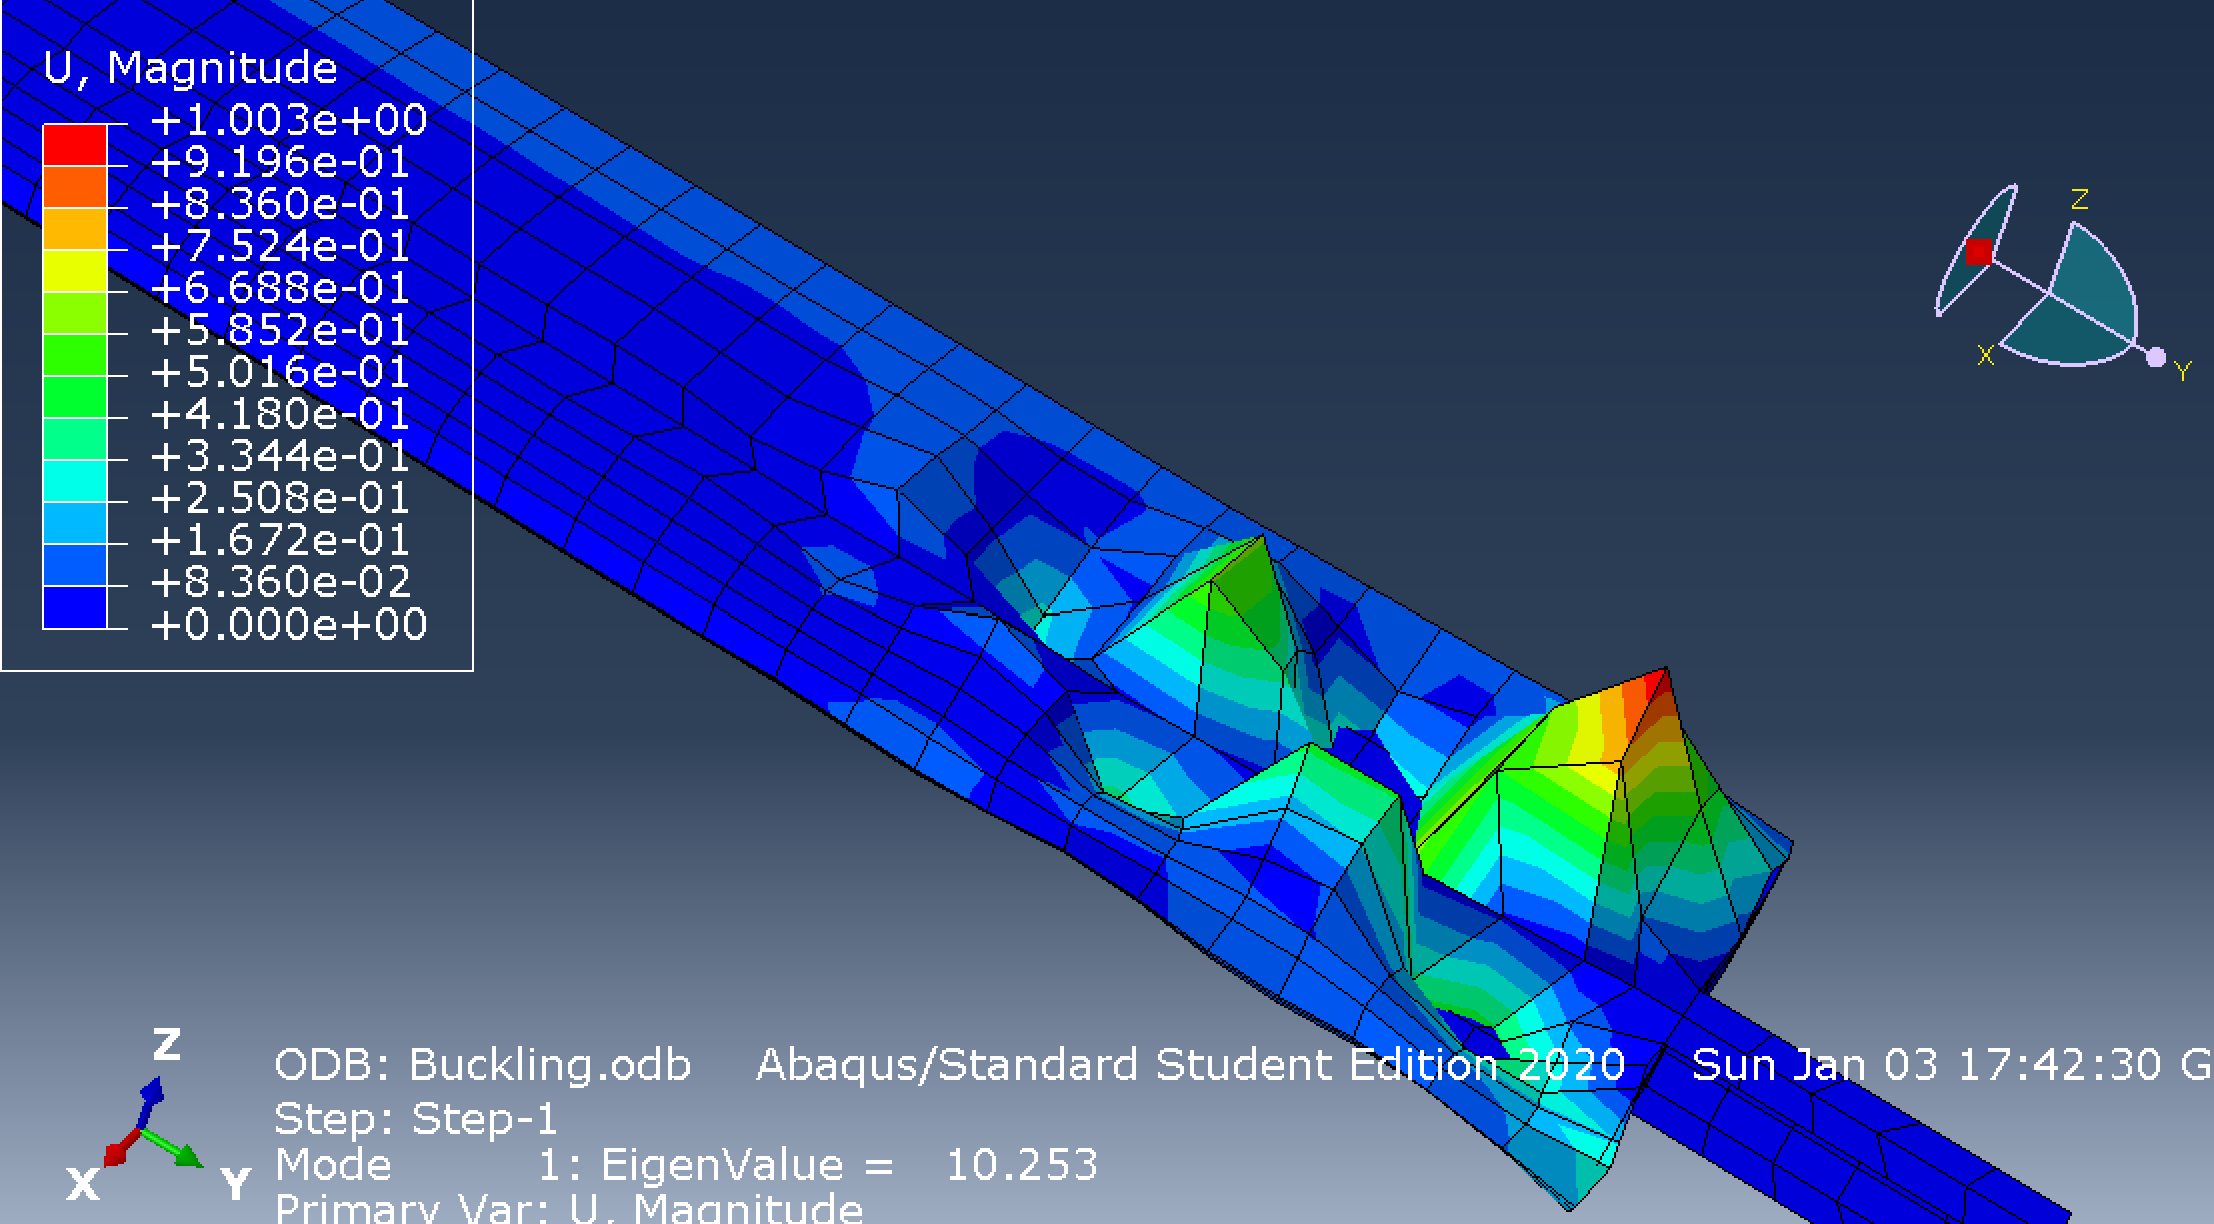
\includegraphics[scale=0.4]{Bilder/Beulen100N}\\
 \label{Beulform}
 \caption{Beispiel Beulform}
\end{figure}
\newpage

 

  
